\documentclass[10pt,fleqn,a4paper]{article}
\usepackage[english]{babel}
\usepackage{graphicx} % plaatjes zijn goed
\usepackage{comment}  % uitcommentarieren van blokken oud spul
\usepackage[hmargin=2.5cm,vmargin=2cm]{geometry} % meer ruimte
\usepackage{amsmath,amssymb,latexsym}
\usepackage{float}
\usepackage{listings}
\lstset{language=Ruby}

\newcommand{\keywords}[1]{\par\addvspace\baselineskip\noindent\enspace\ignorespaces{\textbf{Keywords:~}}#1}
\newcommand{\negmuchspace}{\negthinspace\negthinspace\negthinspace\negthinspace\negthinspace\negthinspace\negthinspace\negthinspace\negthinspace\negthinspace\negthinspace\negthinspace\negthinspace\negthinspace\negthinspace\negthinspace\negthinspace\negthinspace}
\newcommand{\ds}[1]{d^2_{#1}}
\newcommand{\dsa}[1]{\overline{d^2}_{#1}}

%opening
\title{Domain-Specific Questionnaires}
\author{Marten Veldthuis}
\addtolength{\parskip}{0.5\baselineskip}
\allowdisplaybreaks[1]

\begin{document}

\sloppy
\begin{twocolumn}
\twocolumn[
\maketitle
\begin{@twocolumnfalse}
\begin{abstract}
This paper has an abstract. But I will not write the abstract until
the paper is largely done. Makes sense, no?  

\keywords{Domain Specific Languages, Language Design, Ruby, Rails,
  Dynamic Programming, Questionnaires, Psychiatrics, Web-Applications}

\end{abstract}
\vspace{5mm}
\end{@twocolumnfalse}
]

\section{Introduction}
% 1 - context of problem

The Rob Giel Onderzoekscentrum (RGOc) is a research center developing
a product called RoQua. RoQua is a web application which allows
psychiatric departments of health-care providers to monitor patients by
periodically letting them fill out questionnaires over the Internet.

Right now, RoQua uses a third-party web service called GlobalPark to
display, and have patients fill in, the actual questionnaires. While
this is a good separation of concerns for the application, in section
\ref{sec:problems} we will outline the problems with GlobalPark. In
section \ref{sec:approach} we explain our solutions to these problems,
and the rationale behind them.

\section{Problems}\label{sec:problems}
%   - which problem is addressed

GlobalPark is a costly service, and given the nature of the data, the
RGOc would rather not be reliant on a service which is not under its
own control.

Another problem the RGOc is experiencing with the GlobalPark service
is a matter of usability. Defining questionnaires through the web
interface of GlobalPark is a slow process. The web interface for
editing questionnaires is slow, and gets increasingly slower when
there are more questions defined for a questionnaire. 

It's also not possible to define multiple views for the same
questionnaire. In RoQua, this is needed because for most
questionnaires, both a patient-version as well as a bulk-input version
needs to be available. Currently, this means questionnaires have to be
defined twice, both in GlobalPark and in RoQua itself.

Lastly, the way GlobalPark sends back information to RoQua is by doing
an HTTP GET request back to RoQua. This opens up a potential CSRF
security hole. Additionally, this interface contains character
encoding bugs, and GlobalPark is largely unresponsive to bug reports.

All things considered, the RGOc would like to move away from
GlobalPark and switch to a replacement of their own.

\section{Related work}
% 2 - related work
%     - for DSL
%     - for webbased forms: globalpark, netquestionnaire, but also
%       indirect competitors


\section{Goals}

The goals for the project, which was given the name Quby, and will be
referred to as such from here on, are then defined as:

\begin{enumerate}
\item Replace all functionality of GlobalPark, for as far as we use it
  currently.
\item \label{dsl} Make it easier to define questionnaires.
\item \label{restful} Make the API interface with RoQua simpler.
\end{enumerate}


\section{Background of technology}
% - background of technology used Roqua is written using a web
application framework called Ruby on Rails. Given that this framework
provides options for integrating with other Ruby on Rails
applications, Quby will be written in Rails too. Communication between
the two is done by exposing a RESTful web service interface on the
side of Quby, which will output JSON documents.


\section{Architectural Overview}
% 3 - architectural overview (of Quby, and of Quby as a service in its
% setting within Roqua)

Ruby on Rails applications follow a standard Model-View-Controller
pattern.

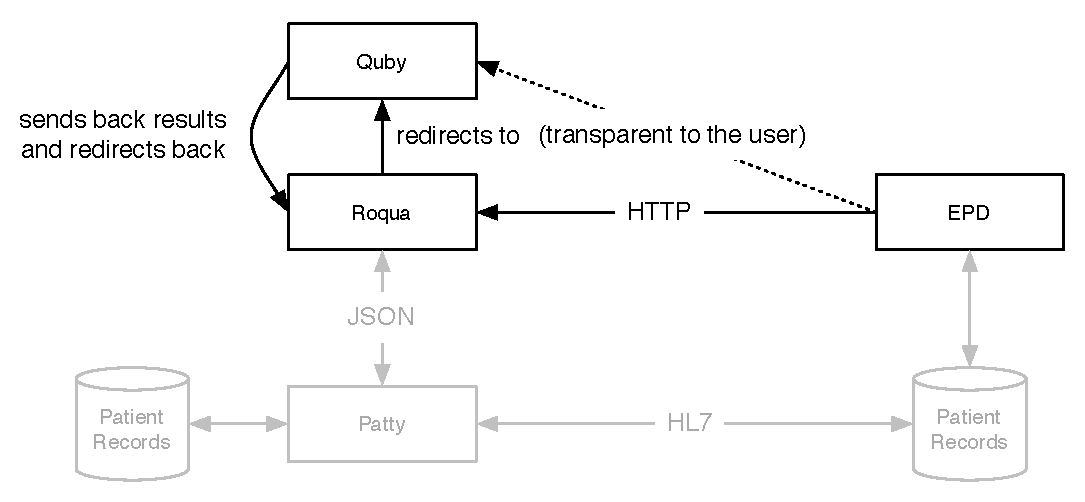
\includegraphics{quby-in-its-setting.pdf}

\subsection{DSL}

One issue traditionnally seen in many Ruby domain-specific languages
is that they tend to pollute the namespace. For instance, take the
following snippet of Rails code:

\begin{lstlisting}
class Sprocket < ActiveRecord::Base
  belongs_to :widget
end
\end{lstlisting}

In this case, \lstinline{belongs_to} is part of the DSL which Rails'
ActiveRecord provides. But it's actually a class method, and if you
try to define your own \lstinline{belongs_to}, you have to be
careful. For Rails, this is usually not that big a problem, given the
naming of the DSL methods they use.

However, with the DSL we wanted to have for Quby, these collisions
would be common. In this paper we will show a method of solving this
problem, without having to consort to Ruby parsetree manipulation
tools, which can be cumbersome to build, maintain and debug.

Our approach is similar in spirit to the Decorator
pattern\cite{Erich:1995design} in that we too have a seperate
Questionnaire\-Decorator class which decorates the Questionnaire
instances at runtime. Implementation-wise, we leverage Ruby's dynamic
nature.

Upon instantiation of a questionnaire object we instantiate a
decorator and evaluate the questionnaire definition within the
decorator instance. Any DSL methods are implemented as instance
methods on the decorator. These DSL methods then modify the
questionnaire object, filling in instance variables such as
\lstinline{@questions}.

\begin{lstlisting}
class Questionnaire
  def initialize(definition)
    QuestionnaireDecorator.decorate(self, definition)
  end
end

class QuestionnaireDecorator
  def self.decorate(destination, definition)
    instance = self.new(destination)
    instance.instance_eval(definition)
  end

  def initialize(destination)
    @destination = destination
  end

  def question(title)
    @destination.instance_eval do
      @questions ||= []
      @questions << title
    end
  end
end
\end{lstlisting}

\section{Implementation}
% 4 - Implementation



\section{Evaluation}
% 5 - evaluation
%     - user evaluation
%     - comparison with tools


\section{Future Work}


\section{Conclusion}
% 6 concluding remarks

We have devised a way of implementing the decorator pattern for a dynamic language. This allows us to easily develop domain-specific languages without code generation, or having to implement our own parser.


%----------------------------------------------------------------------------------
\bibliographystyle{plain}
\bibliography{DomainSpecificQuestionnaires}

\end{twocolumn}

\end{document}
